% !TEX root = approx8.tex


\subsection{Quasi-rigidity and Corollary \ref{cor:quasi-rig}}\label{subsec:qrig-cor}

We start by restating Corollary \ref{cor:quasi-rig} in a more precise way.

\begin{cor}\label{cor:quasi-rig2} Fix  a closed  Riemannian manifold $(N,\mathtt{g})$, its unit cotangent
bundle $D^{\ast}N$ as well as an $\epsilon > 0$.  Fix also a family $\F =\{F_{0},\ldots, F_{l}\}$ of fibres of $D^{\ast}N$ that  $\epsilon$-approximates $\lag^{(ex)}(D^{\ast}N)$,  as constructed in Theorem \ref{thm:nearby}
(see Definition \ref{d:approx-sys}).  Consider an exact symplectomorphism  $\phi :D^{\ast}N\to D^{\ast}N$ with support in the
interior of $D^{\ast}N$ and let
 $$\chi (\phi; \F) =\max_{F\in\F}\ \{ \max h_{\phi(F)} - \min h_{\phi(F)}\}~.~$$
 For any $L\in \mathcal{L}ag^{(ex)}(D^{\ast}N)$, we have $$d_{\gamma}(L,\phi(L)) \leq 4(\epsilon + N(L;\F, \epsilon) \chi(\phi;\F))~.~$$
\end{cor}

We recall that for an exact Lagrangian $L\subset D^{\ast}N$ we denote by $h_{L}:L\to \R$ a choice of a primitive on $L$ for the exact $1$-form $\lambda$. This notation is used for $L\in\lag^{(ex)}(D^{\ast} N)$, for fibers $F$ of $D^{\ast}N$, as well as for Lagrangians such as $\phi(F)$ which coincide with the fiber $F$ outside the support of $\phi$. Notice also that $Var (h_{L})=\max h_{L} - \min h_{L}$ is independent of the choice of primitive $h_{L}$.

\begin{rem}\label{rem:quasi-isom}
a. We refer to the property in the Corollary \ref{cor:quasi-rig2} as  {\em quasi-rigidity} because its meaning is that  the size of the action of $\phi$ on the whole of $\lag^{(ex)}(D^{\ast}N)$ is constrained by that on the finite family of fibers $\F$. In particular, notice that if $\phi(F)=F$ for all the fibers $F\in \F$, then, for such an $F$, $Var(h_{\phi(F)})=0$ and  thus $\chi(\phi;\F)=0$. Therefore, in this case
we have $$d_{\gamma}(L,\phi(L)) \leq 4\epsilon \ \ , \forall \ L\in\lag^{(ex)}(D^{\ast}N)~.~$$

b. In both Corollaries \ref{cor:link2} and \ref{cor:quasi-rig2} there is a factor two 
on the right side of the respective stated inequalities that could be avoided by using in the definition of TPC-approximability the pseudo-metric $D_{\mathrm{int}}$ from  (\ref{eq:d-int3}) instead of $\dint$. 

c. It is likely that in the statement of the corollary it is possible to replace $N(L;\F,\epsilon)$ by
$\# (\F )$, the number of elements in the $\epsilon$-approximating family $\F$.
\end{rem}

\begin{proof}[Proof of Corollary \ref{cor:quasi-rig2}] The argument makes use of the 
Lefschetz fibration $\bar{h}:E\to\mathbb{C}$, the Lagrangian spheres  $\hat{S}_{x_{i}}\subset E$ and  of the setting  leading to the definitions of the local and ambient approximability data  in \S\ref{subsubsec:local_approx_d} and \S\ref{subsubsec:amb_approx_d}, respectively. The construction of $\bar{h}$ and its properties are in \S\ref{subsec:Giroux} and \S\ref{subsec:Lef-Dehn}.  

Given $L\in\lag^{(ex)}(D^{\ast}N)$ there exists an iterated cone $C_{L}$ in the category
$\mathscr{D}_{p}(D^{\ast}N)$ (see \S\ref{subsubsec:amb_approx_d}) as given in equation (\ref{eq:iterated_cones4}) :
\begin{equation}\label{eq:iterated_cones7}
 \Delta_{i} \ : \ Z_{i}\longrightarrow X_{i}\longrightarrow X_{i+1} \ , \ 0\leq i < m \ , 
\end{equation}
with $Z_{j}$ of the form $\Sigma^{l(j)}\hat{S}_{x_{s(j)}}$ or $=0$,
with each $\Delta_{i}$  exact in
 $(\mathscr{D}_{p}(E))^{0}$. Here $X_{0}=0$, 
$C_{L}=X_{m}$,  and there is a Lagrangian $X_{L}$  disjoint from $D^{\ast}N$ such that 
$\dint (L\oplus X_{L},C_{L}) <\epsilon + c_{\epsilon}\nu(p)$ - see  Corollary \ref{thm:nearby_far}. We will also assume that this decomposition is of minimal length, thus $m=N(L;\F,\epsilon)$.

The exact symplectomorphism $\phi$ from the statement naturally extends to $E$ by the identity in the exterior of $D^{\ast}N$. We denote this extension still by $\phi$. Notice that $\phi(X_{L})=X_{L}$.

With these conventions, recall from \S\ref{sbsb:symplecto-fun}, see (\ref{eq:phi-fun-2}) and (\ref{eq:phi-fun-3}), that the symplectic diffeomorphism
$\phi$ induces a TPC functor $\bar{\phi}:=PD(\phi) :\mathscr{D}_{p}(D^{\ast}N)\to \mathscr{D}_{\phi_{\ast}p}(D^{\ast}N)$ (we recall that the space of perturbations $\mathcal{P}$ is closed under the action of $\phi$).  

Denote $L'=L\oplus X_{L}$.  Notice that $\dint(L,\phi(L))= \dint(L\oplus X_{L},\phi (L)\oplus X_{L})$ and the interleaving distance $\dint(X,\phi(L))$ is the same in $D^{\ast}N$ and in $E$ (for a choice of perturbation data $p$ on $E$ that extends the choice on $D^{\ast}N$). Let $p, \phi_{\ast}p \preceq q$.
In $\mathscr{D}_{q}(D^{\ast}N)$ we have the inequality: 
$$\dint(\phi(L'),L')\leq \dint(\phi(L'), \mathcal{H}_{\phi_{\ast}p, q}(\bar{\phi}(C_{L})) )+\dint(\mathcal{H}_{\phi_{\ast}p, q}(\bar{\phi}(C_{L})) ,\mathcal{H}_{p,q}(C_{L}))
+\dint( \mathcal{H}_{p,q}(C_{L}),  L')~.~$$
At the same time we also have
$$ \dint(\phi(L'), \bar{\phi}(C_{L}) ) \leq \dint(L',C_{L}) < \epsilon +c_{\epsilon}\nu(p) $$ 
in $\mathscr{D}_{\phi_{\ast}p} (D^{\ast}N)$
because $\bar{\phi}$ is a persistence functor and therefore non-dilating with respect to $\dint$ (see Lemma \ref{l:d-func} i).
The functors $\mathcal{H}_{p,q}$, $\mathcal{H}_{\phi_{\ast}p,q}$  too are non-dilating  with respect to the respective interleaving pseudo-metrics.
 Thus,  in $\mathscr{D}_{q}(D^{\ast}N)$ we have 
$$ \dint(\phi(L'), \mathcal{H}_{\phi_{\ast}p,q}(\bar{\phi}(C_{L}) )) < \epsilon+c_{\epsilon}\nu(p),\ \dint( \mathcal{H}_{p,q}(C_{L}), L') < \epsilon +c_{\epsilon}\nu(p)~.~$$ 

Starting from this point we  first prove the statement  under the additional 
assumption: \begin{equation}\label{eq:fix_F}
\phi(F)=F \ , \ \forall \ F\in \F ~.~\end{equation}
Under this assumption we first notice that the statement follows if we can show that:
\begin{equation}\label{eq:equality_tr_dist}
\dint (\mathcal{H}_{\phi_{\ast}p, q}(\bar{\phi}(C_{L}), \mathcal{H}_{p,q}(C_{L}))=0
 \end{equation}
 for some $q$ such that $p ,\phi_{\ast}p \preceq q$  by  taking into account the relationships among
$\dint$, $D_{\mathrm{int}}$, and $d_{\gamma}$ as  in equations (\ref{eq:d-int3}), (\ref{eq:ineq_var_inter}) and (\ref{eq:equality_int}) and taking $p$ such that $\nu(p)\to 0$.

We now proceed to justify (\ref{eq:equality_tr_dist}) under  the additional assumption (\ref{eq:fix_F}).
The iterated cone $C_{L}$ belongs to the category 
$$\mathscr{D}_{p}(E)=PD(\fuk(\mathcal{L}ag^{(ex)}(E), p))~.~$$
Recall that there is another model for this category in terms of twisted complexes as 
described in \S\ref{sbsb:ftw} that we will denote by $\mathscr{D}^{Tw}_{p}(E)$.
This TPC  is the persistence homological category of the filtered twisted complexes over
the filtered $A_{\infty}$-category with objects the exact, closed Lagrangians in $E$. With
the notation in \S\ref{sbsb:ftw}:
$$\mathscr{D}^{Tw}_{p}(E)=PH\left(FTw\left(\fuk(\mathcal{L}ag^{(ex)}(E), p) \right)\right).$$
The Yoneda embedding extends to a $0$-equivalence of TPCs:
$$\mathcal{Y}_{p}: \mathscr{D}^{Tw}_{p}(E) \to \mathscr{D}_{p}(E)$$ which is compatible (up to $0$-isomorphism) with the comparison functors $\mathcal{H}_{p,q}$, when $p\preceq q$.
In particullar, the iterated cone $C_{L}$ is $0$-isomorphic to a filtered twisted complex 
$$\bar{C}_{L;p}=(\oplus_{i}Z'_{i}, A_{\bar{C}_{L,p}})$$ 
over the shifted Lagrangian spheres $Z'_{i}=\Sigma^{s_{i}}\hat{S}_{x_{j(i)}}$ that 
appear in the decomposition  (\ref{eq:iterated_cones7}).  Such a twisted complex
is characterized by an upper triangular $m\times m$ matrix, $A_{\bar{C}_{L;p}}$, with elements in $CF (\hat{S}_{x_{j}}, \hat{S}_{x_{s}}; p)$ (up to obvious shifts), as described in \cite{Se:book-fukaya-categ} (see also  the filtered $\lambda$-lemma  in \cite{Bi-Co-Sh:LagrSh} and \S\ref{lambdamap}). 
Here $CF(\hat{S}_{x_{i}}, \hat{S}_{x_{j}}; p)$ is the filtered Floer chain complex of $\hat{S}_{x_{i}}$ and $\hat{S}_{x_{j}}$  computed in $E$ with respect to the perturbation data $p$. To emphasize the dependence on the perturbation data we included $p$ in the notation. 

It is easy to track the effect of $\bar{\phi}$ by using twisted complexes through the push-forward of twisted complexes: this transports the Lagrangians involved by $\phi$, it pushes-forward the perturbation data
$p  \to \phi_{\ast}p$ and sends the matrix $A_{\bar{C}_{L;p}}$ to a matrix
$\phi_{\ast}(A_{\bar{C}_{L;p}})$, element to element, by the obvious transformation:
\begin{equation}\label{eq:ident1}
CF(\hat{S}_{x_{j}}, \hat{S}_{x_{s}}; p)\stackrel{\phi_{\ast}}{\longrightarrow} CF (\phi(\hat{S}_{x_{j}}), \phi(\hat{S}_{x_{s}}); \phi_{\ast} p)= CF(\hat{S}_{x_{j}}, \hat{S}_{x_{s}}; \phi_{\ast}p)
\end{equation}
(where we use our assumption that $\phi$ keeps each $\hat{S}_{x_{i}}$ invariant).
We denote the resulting twisted complex by $\phi_{\ast}(\bar{C}_{L,p})$. It has
the form:
$$\phi_{\ast}(\bar{C}_{L,p})=(\oplus_{i}Z'_{i}, A'_{\phi_{\ast}p})\in FTw\left(\fuk(\mathcal{L}ag^{(ex)}(E), \phi_{\ast}p ) \right) $$
where $A'_{\phi_{\ast}p}=\phi_{\ast}(A_{\bar{C}_{L,p}})$. 

At this point we need to be more precise about the various choices of Floer data for the 
pairs $(\hat{S}_{x_{i}},\hat{S}_{x_{j}})$. Due to the properties of the systems of categories
involved here, as described in \S\ref{s:sys-tpc} and in \S\ref{s:pdfuk}, any such choice that is part of our perturbation data family $\mathcal{P}$  is acceptable for this argument. Similarly, we need to discuss the two relevant continuation functors $\mathcal{H}_{p,q}$ and $\mathcal{H}_{\phi_{\ast}p,q}$. It is useful to revisit Figure \ref{fig:new_fibr}  a part of which is reproduced in 
Figure \ref{fig:new_fibr2} with minor adjustments. 

\begin{figure} [h]
  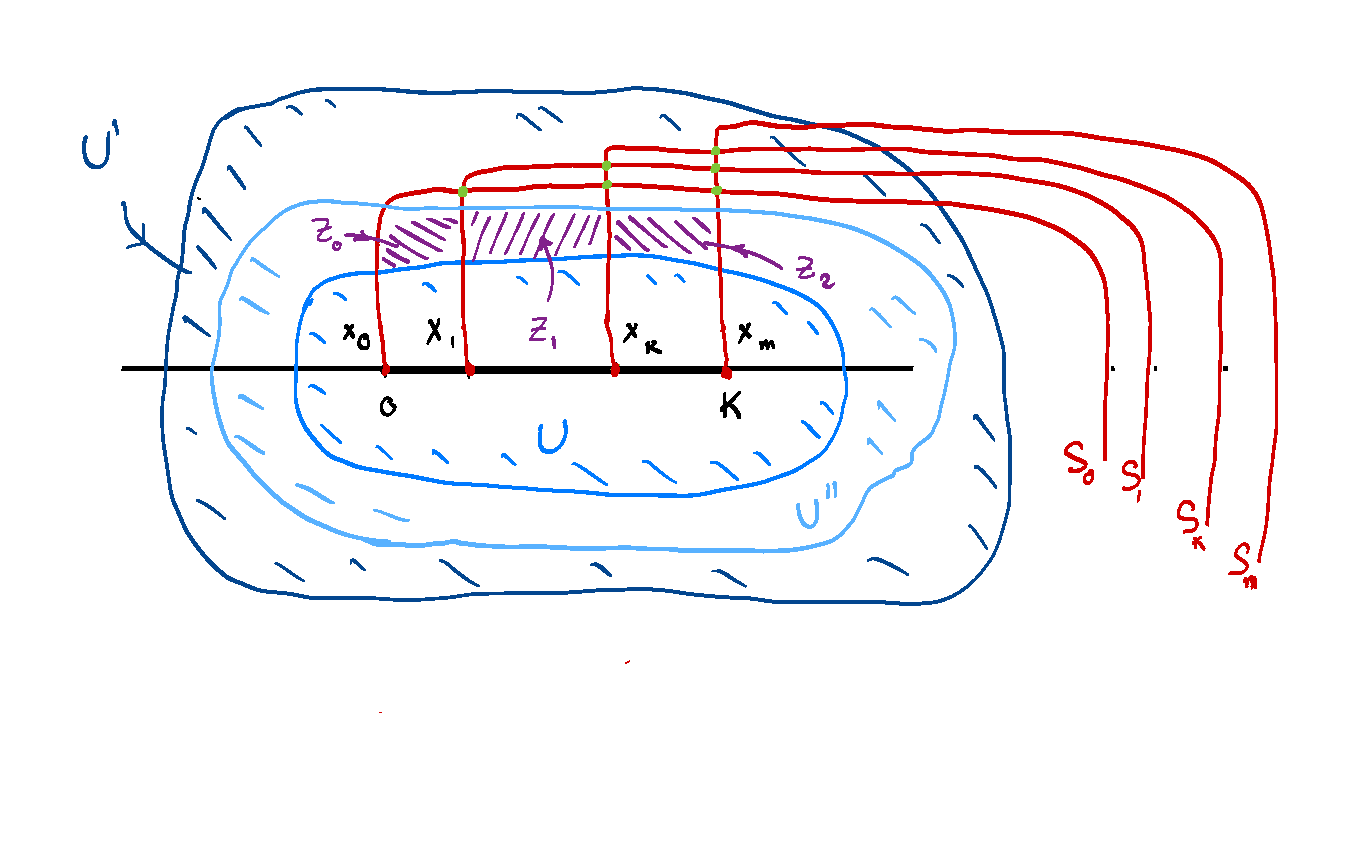
\includegraphics[scale=0.75]{new_fibr2.pdf}
  \centering
  \caption{The Lagrangian spheres and their intersections.} \label{fig:new_fibr2}
\end{figure}
Recall that $U$ in the picture contains the projection onto $\mathbb{C}$ of 
the disk bundle $D^{\ast}N\subset E$ and that the spheres $\hat{S}_{x_{i}}$ can be assumed 
 to coincide with the spheres $S_{x_{i}}$ in the picture outside of $D^{\ast}N$ (this requires slightly modifying some of the $U$, $U'$ in ways irrelevant for the rest of the
 argument). We may also assume that each two spheres $\hat{S}_{x_{i}}$, $\hat{S}_{x_{j}}$
 interesect transversely.  The Floer data for all the pairs $(\hat{S}_{x_{i}},\hat{S}_{x_{j}})$ is chosen such that the Hamiltonian $H^{\hat{S}_{x_{i}},\hat{S}_{x_{j}}}$ is constant outside
 $D^{\ast}N$. Thus the generators of the respective Floer complexes are the intersection points
 between the relevant spheres. The Morse functions on each of the spheres $\hat{S}_{x_{i}}$ are picked to have exactly two critical points, a maximum and a  minimum, both 
 outside $\bar{h}^{-1}(U')$. The almost complex structure $J^{i,j}=J^{\hat{S}_{x_{i}},\hat{S}_{x_{j}}}$ is picked such that $\bar{h}$ is $(J^{i,j}, i)$-holomorphic over $W=\bar{h}^{-1}(U''\backslash U)$. Here, the set $U''$ represents a neighbourhood of $D^{\ast}N$ that is smaller than $U'$, we could take it as the projection of $D^{\ast}_{2}N$, and such that all the intersection points of the Lagrangian spheres $\hat{S}_{x_{i}}$ are outside $U''$.  Further choices of almost complex structures on $E$ used to define 
 higher operations as well as the continuation maps $\mathcal{H}_{p,q}$ and $\mathcal{H}_{\phi_{\ast}p,q}$ are from the same class, in the sense that they make the projection $\bar{h}$ holomorphic. 

With these choices a simple application of the open mapping theorem shows that there are no Floer strips (or even polygons) that have as inputs intersection
points of paris of distinct $\hat{S}_{x_{i}}$, have output at another such intersection point, have boundaries on (some of) these spheres,  and that intersect the region $U''\backslash U$. For instance, if one such curve would intersect the region $Z_{1}$ in the picture it is easy to see that it also would have to extend to the regions $Z_{0}$ and $Z_{2}$ and, by pursuing this argument, one reaches a contradiction.

Recall that the support of $\phi$ is inside $D^{\ast}N\subset \bar{h}^{-1}(U)$. This means
that in fact $\bar{C}_{L,p}$ coincides with $\phi_{\ast}(\bar{C}_{L,p})$ - the two matrixes $A'_{\phi_{\ast}p}$ and $A_{\bar{C}_{L,p}}$ coincide. Moreover, 
again because the Floer type strips or polygons can not cross the region $U''\backslash U$,
is follows that, with obvious choices of perturbation data,  $\mathcal{H}_{p,q}$ and $\mathcal{H}_{\phi_{\ast}p,q}$ act in the same way on $\bar{C}_{L,p}$ and $\phi_{\ast}(\bar{C}_{L,p})$. 
Therefore,
$$\dint (\mathcal{H}_{p,q}(\bar{C}_{L,p}), \mathcal{H}_{\phi_{\ast}p, q}(\phi_{\ast}(\bar{C}_{L,p})))=0$$
which implies  (\ref{eq:equality_tr_dist}) and concludes the proof under the additional assumption (\ref{eq:fix_F}).



We now drop this assumption (\ref{eq:fix_F}) and consider the general case. Our aim is to show

\begin{equation}\label{eq:equality_tr_dist2}
\dint (\mathcal{H}_{\phi_{\ast}p, q}(\bar{\phi}(C_{L}), \mathcal{H}_{p,q}(C_{L}))\leq 
2m \chi(\phi;\F)~.~
 \end{equation}
which is sufficient to end the proof of the Corollary.
Denote $\bar{S}_{i}=\phi(\hat{S}_{x_{i}})$. These are exact Lagrangians spheres with the 
property that $\bar{S}_{i}$ coincides with $\hat{S}_{x_{i}}$ outside $D^{\ast}N$ and are so that the $\bar{S}_{i}$'s are pairwise disjoint inside $D^{\ast}N$. 
As a result, the same argument used under the assumption (\ref{eq:fix_F}) also
shows in the current more general context that the matrix $A'_{\phi_{\ast}p}$ that defines the twisted complex 
$$\phi_{\ast}(\bar{C}_{L,p})=(\oplus_{i}\phi(Z'_{i}), A'_{\phi_{\ast}p})\in FTw\left(\fuk(\mathcal{L}ag^{(ex)}(E), \phi_{\ast}p ) \right ) $$
is identified as a linear map - without taking into account filtrations - 
to $A_{\bar{C}_{L,p}}$ under the transformation $\hat{S}_{x_{i}}\to \bar{S}_{i}$ (that is akin to a basis change). However, the elements of the $m \times m$ matrix $A'_{\phi_{\ast}p}$ have potentially different filtration levels compared to  $A_{\bar{C}_{L},p}$. To understand this change 
notice that the filtered complex $CF(\bar{S}_{i}, \bar{S}_{j})$ is isomorphic to
$\Sigma^{k_{i,j}}CF (\hat{S}_{x_{i}}, \hat{S}_{x_{j}})$ where $|k_{i,j}|\leq Var(h_{\phi(F_{x_{i}})}) +Var(h_{\phi(F_{x_{j}})}) \leq 2\chi(\phi;\F)$. These shifts cumulate and given that we have $m$ terms in the twisted complexes under consideration we deduce (\ref{eq:equality_tr_dist2}) which concludes the proof.
\end{proof}



\subsection{Lagrangian Gromov width and Corollary \ref{cor:link}}\label{subsec:Gw-cor}

We start by recalling the definition of the Gromov width (\cite{Bar-Cor:Serre}, \cite{Bar-Cor:NATO}) that is relevant here. For this consider a symplectic manifold
$(M,\omega)$, a Lagrangian submanifold $L\subset M$ and a closed subset $K\subset M$. The {\em Gromov width of 
$L$ relative to $K$} is defined by:
\begin{eqnarray*}\mathscr{W}(L; K)=\sup \Bigl\{ \pi \frac{r^{2}}{2} \ | \ \exists\  j: (B_{r}, \omega_{0})\to (M,\omega) , \  j \ \text{is an embedding}, \\ j^{\ast}\omega=\omega_{0}, \ \ j^{-1}(L)= B_{r}\cap \R^{n}, \ j(B_{r})\cap K=\emptyset \Bigr\} 
\end{eqnarray*}
where $(B_{r},\omega_{0})\subset (\mathbb{C}^{n},\omega_{0})$ is the standard symplectic $r$-ball in $\mathbb{C}^{n}$, centred at the origin. 

The aim of this subsection is to show Corollary \ref{cor:link}.  
We reformulate here this corollary in a more precise way.

\begin{cor}\label{cor:link2} 
Assume that $(\mathcal{L}ag (M), d_{\gamma})$ is TPC retract $\epsilon$-approximable  in the sense of Definition \ref{d:approx-sys-ret}  in the system $\widehat{\msc}$ of  Fukaya type TPCs, by the  familiy $\F_{\epsilon}$ such that each element of $\F_{\epsilon}$ is a Yoneda module. 
For each $L\in \lag(M)$ we have
$$\mathscr{W}(L;  \cup_{F\in \F_{\epsilon}}F)\leq 2\epsilon ~.~$$\end{cor}



\begin{rem}\label{rem:width-fibers}
a. Corollary \ref{cor:link2} does not directly apply to the case of $M=D^{\ast}N$ because the $\epsilon$-generating 
families $\F_{\epsilon}$ consist  of modules $\mathscr{F}_{x_{i}}$ that correspond to fibers $F_{x_{i}}$ 
but that are not Yoneda modules in the categories $\msc_{p}$ (these are part of the local approximating 
data $(\Phi, \F_{\epsilon})$ - see \S\ref{subsubsec:local_approx_d}).
However, the Corollary does apply to the ambient approximating data $(\Phi',\F'_{\epsilon})$ from \S\ref{subsubsec:amb_approx_d} because, in this case, the elements of $\F'_{\epsilon}$ are represented
by Lagrangian spheres $\hat{S}_{x_{i}}\subset E$. Therefore, recalling $F_{x_{i}}=\hat{S}_{x_{i}}\cap D^{\ast}N$, we deduce that the conclusion of the Corollary remains valid in the case of $M=D^{\ast}N, \ \F_{\epsilon}=\{ F_{x_{1}},\ldots, F_{x_{l}}\}$.


b. The inequality in the statement immediately implies that, when $\epsilon\to 0$, the family $\F_{\epsilon}$ becomes dense in $M$. Indeed, assume that a family $\mathcal{F}_{\epsilon}$ avoids some  ball 
$B\subset M$. Take $L$ that passes through the center $x$ of this ball and also pick an embedding 
$j$, as in the definition of width, with $j(0)=x$ and such that $j(B_{r})\subset B$. We deduce in this case that 
$\epsilon \geq \pi\frac{{r}^{2}}{2}$ and therefore $\epsilon$ is bounded away from zero under the hypothesis
that $\F_{\epsilon}$ does not intersect $B$.

c. In this remarks consider the case $M=D^{\ast}N$. A fiber is determined 
by its base point, and the disk bundle $D^{\ast}N$ is determined by the Riemannian metric $\mathtt{g}$. In view of this,  the Corollary indicates that there are some symplectic invariants associated with pairs $(\mathcal{S},\mathtt{g})$ where $\mathcal{S}$ is a configuration of $k$ distinct points in the base. To see this, for any finite 
family $\mathcal{S}\in N$ denote by $\mathcal{F}_{\mathcal{S}}$ the corresponding family of fibers inside $D^{\ast}N$ (the metric defining the disk bundle being $\mathtt{g}$). Now define the {\em approximability precision} of $\mathcal{S}$ by:
$$\epsilon_{\mathcal{S}}= \inf \{\  \epsilon > 0 \ | \  \mathrm{there\ exists}\ \epsilon-\mathrm{approximating\ data} \ (\Phi, \mathcal{F}_{\mathcal{S}}) \ \mathrm{as\ in}\  \S\ref{subsubsec:local_approx_d} \ \}~.~$$
This is non-zero, by point b, and it is finite. Indeed,  for $\mathcal{S}$ consisting of  a single point, it follows from the arguments in \cite{Bi-Co:mspectral} (which are partially a precursor to the proof of Theorem \ref{thm:nearby}) that $\epsilon_{\mathcal{S}}$ is already finite. This quantity is, obviously, independent of the point in question and is an upper bound for all $\epsilon_{\mathcal{S}}$, for arbitrary finite $\mathcal{S}$. However, for $\mathcal{S}$ with more than a single element this number generally depends on the placement of the points in $N$. For instance, by taking $\mathcal{S}\subset D$ with $D\subset N$ a small disk, $\epsilon_{\mathcal{S}}$ certainly will stay away from $0$ (again by point b),
independently of the number of elements in $\mathcal{S}$. 
But, if the same number of fibers are more uniformly distributed along $N$, then, by increasing the number of elements of $\mathcal{S}$ one can make choices such that $\epsilon_{\mathcal{S}}\to 0$ because, by Theorem \ref{thm:nearby},  $\epsilon$-approximating data exists for all $\epsilon$. We will not pursue this topic here but it obviously warrants more
study.
% Define for each natural number $k$ the following quantity:
%$$\mathrm{app}(k)=\inf \{ \ \epsilon_{\F} \ | \ \F \ \mathrm{is\ a\ finite\ family\ containing}\ k \ \mathrm{ fibers\ of}\ D^{\ast}N \ \}~.~$$
%Thus, this infimizes the approximability precision achievable with $k$ generators. Finally, a family of $k$ fibers $\F$ is
%symplectically equidistributed if $$\epsilon_{\F}=\mathrm{app}(k)~.~$$
%
\end{rem}



\begin{proof}[Proof of Corollary \ref{cor:link2}] The proof follows directly from Corollary 6.13 i.  in \cite{Bi-Co-Sh:LagrSh}. We only need to relate the notation and conventions in that paper to the context here. The first remark is that \cite{Bi-Co-Sh:LagrSh} works in the setting of weakly-filterered $A_{\infty}$ categories. The setting in the current paper
is that of filtered $A_{\infty}$ categories and thus the results and arguments in \cite{Bi-Co-Sh:LagrSh} apply here too.  
Denote the  TPCs in the system $\widehat{\msc}$ by $\msc_{p}(M)$. Take $L\in\lag(M)$. 
Recall from Remark \ref{rem:relation-TPCapp} that there is no difference whether we use $\sdint$ or 
$\dint$ in the definition of retract approximability. Moreover, from the description of $\sdint$ 
in Lemma 4.2.3, we deduce that there exists an element $a\in \Ob(\msc_{p}(M))$, a cone decomposition
$\eta: 0\cobto a$ with linearization in $\F_{\epsilon}$, and a couple of maps $\alpha\in \hom^{r_{1}}(L, a)$, $\beta\in \hom^{r_{2}}(a,L)$ such that $\beta\circ \alpha = i_{0,r_{1}+r_{2}}(id_{L})$ with $r_{1}+r_{2} < 2\epsilon +c_{\epsilon}\nu(p)$ where $p\in\mathcal{P}$ is
a choice of approriate perturbation data. By inspecting the definition of the quantity $\rho$ in (6.16) in \cite{Bi-Co-Sh:LagrSh} we see 
that $\rho(\alpha) < 2\epsilon + c_{\epsilon}\nu(p)$ (in brief, this $\rho(\alpha)$ infimizes $r_{1}+r_{2}$ such that there is a morphism $\beta$ as before). Moreover, this means that, for $\nu(p)$ small enough, we have, 
with the notation in \cite{Bi-Co-Sh:LagrSh}, $w_{p}( (\alpha, a,\eta)) < 2\epsilon +c_{\epsilon}\nu(p)$ (this $w_{p}$ in (6.19)
\cite{Bi-Co-Sh:LagrSh} is a measurement assigned to triples $(\alpha, a, \eta)$ that infimizes $\rho (\alpha)$ over all choices of $\alpha : L\to a$; it also depends on the perturbation data $p$).  From 
Corollary 6.13. i \cite{Bi-Co-Sh:LagrSh} we 
deduce $2\epsilon \geq \frac{1}{2}\delta (L; \cup_{F\in \F_{\epsilon}}F)$. The quantity $\delta (-;-)$
defined on p. 85 in \cite{Bi-Co-Sh:LagrSh} is the double of the Gromov width as defined here, at the beginning of 
this section. This concludes the proof of the corollary.   
\end{proof}

\begin{rem}\label{rem:direct_cor}
 a. As mentioned in the introduction,  there are some purely geometric implications of  Corollaries \ref{cor:quasi-rig2} and \ref{cor:link2} that are independent of approximability as well as of
 the machinery used for their proofs.  The first statement can be  read as saying that for each $\epsilon>0$ there exists a finite  family of Lagrangians in the class providing approximations (fibers for $T^{\ast}N$, equators for $S^{2}$ etc)   such that the Gromov width of any $L\in \lag^{(ex)}(M)$ relative to this family is less than $\epsilon$. Similarly, focusing on the case of $M=D^{\ast}N$, for any $\epsilon>0$ there exists a finite family of fibers $\F$ such that any exact symplectic diffeormorphism  satisfying $\phi(F)=F$ for all $F\in\F$  only moves each $L\in \lag^{(ex)}(D^{\ast}N)$ less than $\epsilon$ in the spectral metric. 
 
 b. Some of these geometric consequences can also be obtained by more direct means. Indeed, 
 it was noticed by Egor Shelukhin that for any $\epsilon>0$ one can prove by methods unrelated to Fukaya category techniques  that there exists a finite family $\F$ of fibers of $D^{\ast}N$ such that any  Hamiltonian diffeomorphism $\phi$ induced by a Hamiltonian isotopy with support inside $D^{\ast}N$ and disjoint from the fibers in $\F$, has spectral 
 norm smaller than $\epsilon$.  The proof uses the same type of  Morse functions $\varphi$ as constructed in Proposition \ref{prop:Morse} and a result of Usher \cite{Ush10}. This result also implies
 that the Gromov width of the complement of the fibers inside $D^{\ast}M$ can be bounded above by $\epsilon$. This Gromov width  result was also noticed by Mark Gudiev by means of a direct displacement argument using the Morse functions $\varphi$ as in Proposition \ref{prop:Morse}.
\end{rem}

% !TEX root = approx8.tex



\subsubsection{Gromov width, cone length and sizes of approximating
  families} \label{sbsb:gwidth-2}

Let $(M, \omega)$ be a symplectic manifold of one of the types
described in~\S\ref{s:pdfuk} and let $\lag$ be a subset of the
collection of Lagrangians in $M$, as in~\S\ref{sb:sys-fuk}. Recall
that we have the system of filtered $A_{\infty}$-categories
$\widehat{\fuk}(\lag)$ and its filtered derived system of TPC's
$PD(\widehat{\fuk}(\lag))$.

Let $\mathcal{S}$ be a collection of subsets of $M$ and
$\mathcal{L} \subset \lag$ a collection of Lagrangians from
$\lag$. For $w > 0$ define the $w$-density index of $\mathcal{S}$
relative $\mathcal{L}$ to be:
\begin{equation} \label{eq:density-rel} I(\mathcal{S}, \mathcal{L}; w)
  := \inf \bigl\{k \geq 1 \mid \exists \, S_1, \ldots, S_k \in
  \mathcal{S} \text{ such that } \mathscr{W}(L; S_1 \cup \cdots \cup
  S_k) \leq w, \; \forall L \in \mathcal{L} \bigr\}.
\end{equation}
Here and elsewhere in the paper we use the convention that
$\inf \emptyset = \infty$, $\sup \emptyset = -\infty$. Therefore if
$L \subset S_1 \cup \cdots \cup S_k$ for some $L \in \lag$,
$S_1, \ldots, S_k \in \mathcal{S}$, then we have
$\mathscr{W}(L; S_1 \cup \cdots \cup S_k) = -\infty$ hence
$\mathscr{W}(L; S_1 \cup \cdots \cup S_k) \leq w$ is automatically
satisfied in~\eqref{eq:density-rel}.

For a subset $\mathcal{K} \subset \lag$ we denote by
$$\widetilde{\mathcal{K}} \subset
\widetilde{\Ob}(PD(\widehat{\fuk}(\lag)))$$ the collection of
equivalence classes (see~\S\ref{s:approximability}) of the objects
$\mathcal{Y}_p(K) \in \Ob(PD(\fuk(\lag; p)))$, $K \in \mathcal{K}$,
$p \in \mathcal{P}$, where
$\mathcal{Y}_p: \fuk(\lag; p) \longrightarrow F\md_{\fuk(\lag; p)}$ is
the Yoneda embedding (see~\S\ref{gio:fyon-def}
and~\S\ref{sbsb:yoneda-sys}).

The following is an immediate consequence of
Corollary~\ref{cor:link2}.
\begin{cor} \label{c:approx-index} Let
  $\mathcal{L}, \mathcal{F} \subset \lag$ be two collections of
  Lagrangians. Let $w_0 > 0$ and $\mathcal{F}^0 \subset \mathcal{F}$
  be a finite subset such that $\widetilde{\mathcal{L}}$ is
  $w_0$-retract-approximable by $\widetilde{\mathcal{F}^0}$ in
  $PD(\widehat{\fuk}(\lag))$. Then
  \begin{equation} \label{eq:size-index} |\mathcal{F}^0| \geq
    I(\mathcal{F}, \mathcal{L}; w_0).
  \end{equation}
  Moreover, there exists $L \in \mathcal{L}$ such that
  $N^r(L; \widetilde{\mathcal{F}^0}, w_0) \geq I(\mathcal{F},
  \mathcal{L}; w_0)$.
\end{cor}

\begin{rems} \label{r:approx-index}
  \begin{enumerate}
  \item Point (a) of Remark~\ref{rem:width-fibers} applies here as well.
    Namely, the conclusion of Corollary~\ref{c:approx-index} continues
    to hold for $M = D^*N$ with $\mathcal{L} = \lag$ being the
    collection of all closed exact Lagrangians in $D^*N$ and with
    $\mathcal{F}$ being any collection of cotangent fibers.
  \item If $\mathcal{S}' \subset \mathcal{S}''$,
    $\mathcal{L}' \supset \mathcal{L}''$, $w' \leq w''$, then
    \begin{equation} \label{eq:ineq-index} I(\mathcal{S}', \mathcal{L}';
      w') \geq I(\mathcal{S}'', \mathcal{L}'';w'').
    \end{equation}
    In particular, for every $\mathcal{S}$ and $\mathcal{L}$ we have
    $I(\mathcal{S}, \mathcal{L}; w) \geq I(\mathcal{S}, \emptyset;
    w)$. Note that the latter invariant depends on the collection
    $\mathcal{S}$ itself and does not involve any Lagrangian
    submanifolds.
  \item The inequality~\eqref{eq:size-index} may become useful if we
    fix a collection $\mathcal{F}$ that (retract) approximates
    $\mathcal{L}$ and want to bound from below the size of any
    possible finite family $\mathcal{F}^0 \subset \mathcal{F}$ that
    retract-$w_0$-approximates $\mathcal{L}$. Note that there is
    no particular assumption on the collection of Lagrangian $\mathcal{F}$
    in Corollary~\ref{c:approx-index}, besides containing
    $\mathcal{F}^0$ (and being a subset of $\lag$ of course). In
    particular we do not even need assume that $\mathcal{F}$ retract
    approximates $\mathcal{L}$. But in view of~\eqref{eq:ineq-index}
    the most effective bounds from below in~\eqref{eq:size-index} on
    $|\mathcal{F}^0|$ are obtained when $\mathcal{F}$ is minimal as
    possible and in applications it makes sense to assume that
    $\mathcal{F}$ retract approximates $\mathcal{L}$.
  \end{enumerate}
\end{rems}

Here is a simple example showing how Corollary~\ref{c:approx-index}
can be used in practice. Consider $M=S^2$ endowed with its standard
symplectic structure $\omega$ normalized such that
$\text{Area}(S^2, \omega) = 1$. Let $\lag$ be the collection of all
closed monotone Lagrangian in $S^2$ (in this case, all the embedded
closed curves which separate $S^2$ into two domains of area
$\tfrac{1}{2}$). Let $\mathcal{F} \subset \lag$ be the collection of
all great circles passing through the north and south poles of $S^2$.
By Proposition~\ref{OCS2}, $\widetilde{\mathcal{F}}$
retract-approximates $\widetilde{\lag}$ in $PD(\widehat{\fuk}(\lag))$.

We claim that
$I(\mathcal{F}, \emptyset; w) \geq \lceil \tfrac{1}{4w}
\rceil$. Indeed, if $F_1, \dots, F_k \in \mathcal{F}$ then at least
one of the connected components of
$S^2 \setminus (F_1 \cup \cdots \cup F_k)$ must have area
$\geq \tfrac{1}{2k}$ hence
$\mathcal{W}(\emptyset; F_1 \cup \cdots \cup F_k) \geq \tfrac{1}{4k}$.
It follows that
$I(\mathcal{F}, \emptyset; w) \geq \lceil \tfrac{1}{4w} \rceil$. (In
fact, it is not hard to see that we have equality here.)

It follows from Corollary~\ref{c:approx-index} that for every
$\mathcal{L} \subset \lag$, every $w_0>0$, and every finite collection
$\mathcal{F}^0 \subset \mathcal{F}$ which $w_0$-retract-approximates
$\mathcal{L}$ we have:
$$|\mathcal{F}^0| \geq I(\mathcal{F}, \mathcal{L}; w_0) \geq
I(\mathcal{F}, \emptyset; w_0) \geq \Bigl\lceil \frac{1}{4w_0} \Bigr
\rceil.$$
